\documentclass[12pt,a4paper]{article}
\usepackage[UTF8]{ctex} % 支持中文
\usepackage{geometry}
\usepackage{graphicx}
\usepackage{amsmath}
\usepackage{float}
\usepackage{subfigure}
\usepackage{booktabs} % 表格美化
\usepackage{cite}
\usepackage{ulem}
\usepackage{array}
\usepackage{multirow}

\newcolumntype{M}[1]{>{\centering\arraybackslash}m{#1}}
\newcommand{\down}[2]
{
	$#1_{#2}$
}

% 设置页面边距
\geometry{left=2.5cm,right=2.5cm,top=2.5cm,bottom=2.5cm}

\title{\Huge{\textbf{\uuline{实\ 验\ 报\ 告}}}}
\author{\uline{少年班}\ 学院 \quad 姓名:\ \uline{顾泓宇} \quad 学号:\ \uline{PB23000078} \quad 实验日期:\ \uline{2024-2-6} }
\date{}

\begin{document}
	\maketitle
	
	\section{实验题目}
	半导体温度计的设计和制作
	
	\section{实验目的}
	进一步理解热敏电阻的伏安特性和惠斯通电桥测电阻的原理，学习非电学量的电测法，了解实验中的替代原理的应用，同时提高组装、焊接电路的操作能力。
	
	\section{实验仪器}
	热敏电阻、待焊接的电路板、微安表、电阻器、电烙铁、电阻箱、电池、导线、万用表、恒温水浴
	
	\section{实验原理}
	半导体温度计就是利用半导体的电阻值随温度变化而发生急剧变化的特性而制作的，以半导体热敏电阻为传感器，通过测量其电阻值来确定温度的仪器。一般使用金属氧化物半导体作温度传感器。\\
	热敏电阻的伏安特性曲线和测温电路原理图如下：\\
	\begin{center}
	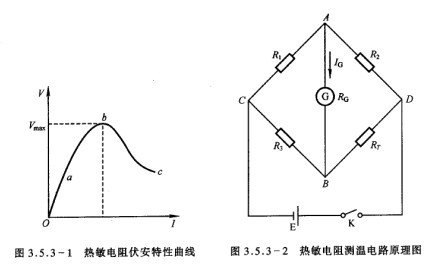
\includegraphics{1.jpg}\\
	图一：热敏电阻的伏安特性曲线和测温电路原理图
	\end{center}
	当取伏安特性曲线的a段时，近似认为符合欧姆定律。当$I_{G}$使G满偏时，近似认为$V_{CD}=I_{T}(R_{3}+R_{T})$.由基尔霍夫方程组解得：\\
	$R_{1}=\frac{2V_{CD}}{I_{G}}(\frac{1}{2}-\frac{R_{T2}}{R_{T1}+R_{T2}})-2(R_{G}+\frac{R_{T1}R_{T2}}{R_{T1}+R_{T2}})$\\
	由上式可以确定$R_{1}(=R_{2})$,其中$R_{3}$的确定是在下限温度电阻$R_{T1}$下，使电桥平衡，从而有$R_{3}=R_{T1}$,$R_{2}=R_{1}$.由下表可以知道，$R_{3}=R_{T1}=2277\Omega$,$R_{T2}=462\Omega$.作出$R-T$曲线并计算得：$R_{1}=R_{2}=4545\Omega$.
	\begin{center}
		\begin{tabular}{|M{4em}|M{4em}|M{4em}|M{4em}|M{4em}|M{4em}|M{4em}|M{6em}|}\hline
			T(\textdegree C) & 15.0 & 20.0 & 25.0 & 30.0 & 35.0&40.0 & 45.0\\
			\hline
			R($\Omega$) & 2750 & 2277 & 1922 & 1654 & 1388 & 1186 & 1004 \\
			\hline
			T(\textdegree C) & 50.0 & 55.0 & 60.0 & 65.0 & 70.0 & 75.0 & $R_{G}=3970\Omega$ \\
			\hline
			R($\Omega$) & 860 & 730 & 623 & 537 & 462 & 403 & $I_{G}=50\mu a$ $U_{CD}=1V$ \\
			\hline

		\end{tabular}
		表一：热敏电阻的R-T关系和基本实验条件
	\end{center}
	\begin{center}
	\scalebox{0.5}{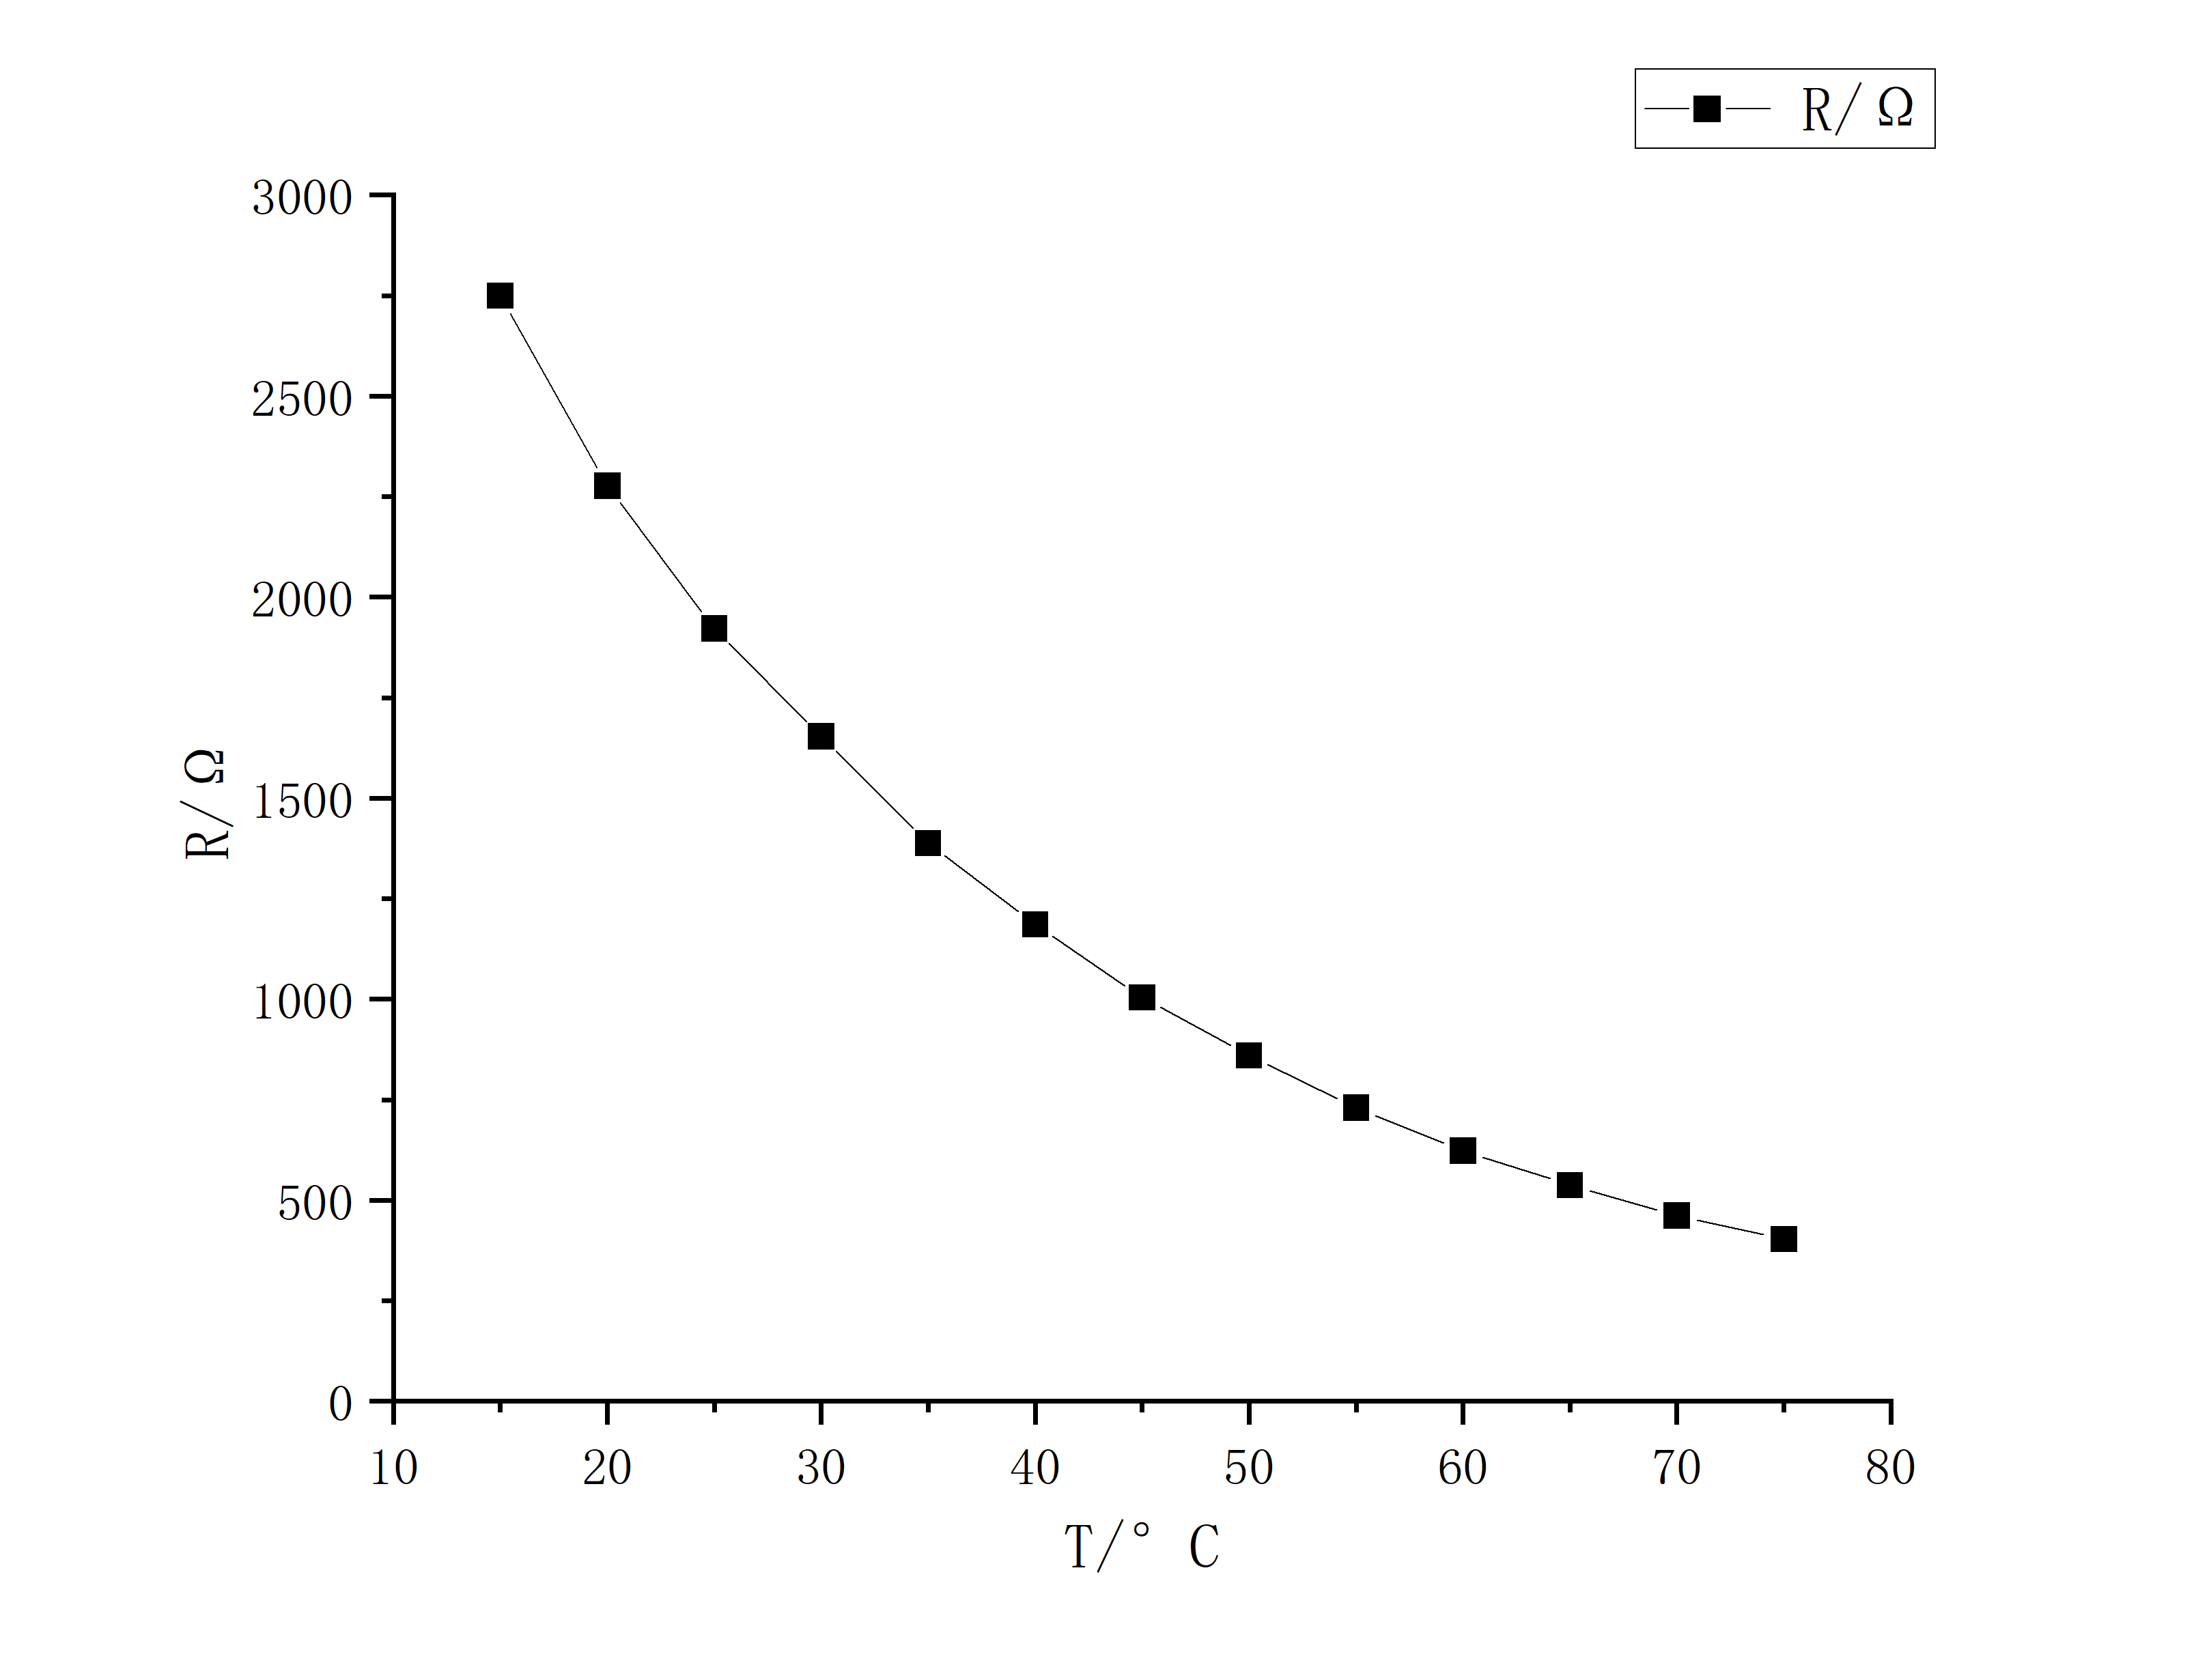
\includegraphics{2.jpg}}\\
	图二：T—R关系图
	\end{center}
	
	\subsection{实验内容}
	\hangindent=1.3cm \hangafter=1
	\quad (1)在坐标纸上绘出热敏电阻的电阻-温度曲线，确定所设计的半导体温度计的下限温度（ 20 \textdegree C）所对应的电阻值$R_{T1}$和上限温度(70\textdegree C)所对应的电阻值$R_{T2}$。再由热敏电阻的伏安特性曲线确定最大工作电流$I_{T}$。根据实验中采用的热敏电阻的实际情况，选取\down{V}{CD}=1V，它可以保证热敏电阻工作在它的伏安特性曲线的直线部分。\\
	\quad (2)令$R_{3}$=$R_{1}$，即测量温度的下限电阻值，由式（3）计算出桥臂电阻$R_{1}$和$R_{2}$的电阻值。式中$R_{T2}$为量程上限温度的电阻值；$R_{G}$为微安表的内阻。\\
	\quad
	(3)熟悉线路原理图（图3.5.3-2）和底版配置图（图3.5.3-4），对照实验所用元件、位置及线路的连接方向。\\
	\quad
	(4)注意正确使用电烙铁，学会焊接，防止重焊、虚焊、漏焊、断路。焊接时K1放在1挡，电流计“+”端与E处要最后连接，以免损坏电表。\\
	\quad
	(5)标定温度计,\down{R}{1}和\down{R}{2}的调节和测量：开关置于1挡，拨下E处接线，断开微安计，用多用表检查\down{R}{1}和\down{R}{2}，使之阻值达到式（3）的计算值（可以取比计算值略小的整数）。
	\begin{center}
		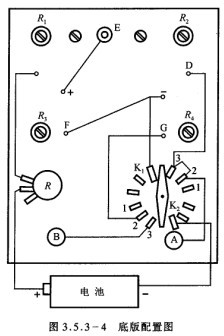
\includegraphics{3.jpg}\\
	\end{center}
	
	
	\subsection{数据分析}
	实验所测量得到的结果如下：
	\begin{center}
		\begin{tabular}{|M{6em}|M{6em}|M{6em}|M{6em}|M{6em}|M{6em}|}\hline
			区域起始/s & 区域末尾/s & 区域中点 & 频数 & 相对频数/\% & 累积频数/\% \\\hline
			5.24 & 5.26 & 5.25 & 3 & 2.0 & 2.0 \\\hline
			5.26 & 5.28 & 5.27 & 5 & 3.3 & 5.3 \\\hline
			5.26 & 5.28 & 5.27 & 5 & 3.3 & 5.3 \\\hline
			5.26 & 5.28 & 5.27 & 5 & 3.3 & 5.3 \\\hline
			5.26 & 5.28 & 5.27 & 5 & 3.3 & 5.3 \\\hline
			5.26 & 5.28 & 5.27 & 5 & 3.3 & 5.3 \\\hline
			5.26 & 5.28 & 5.27 & 5 & 3.3 & 5.3 \\\hline
		\end{tabular}
	\end{center}
	
	\section{结论}

	
	\section{参考文献}
	\bibliographystyle{plain}
	\bibliography{references} % 引用文件名为references.bib
	
\end{document}

